%=== CHAPTER ONE (1) ===
%=== INTRODUCTION ===

\chapter{Introduction}
\begin{spacing}{2.0}
%\setlength{\parskip}{0.2in}

In this section, \textbf{you}, the Student, are expected to state clearly:
%An alphabetcial list of items. Change the \alph* to \Alph* or \roman*
\begin{enumerate}[label=(\alph*)]
    \item the `problem’ or `question’ being researched;
    \item why this topic was chosen;
    \item what motivated the you to choose this topic;
    \item why did you investigate the topic the way you did;
    \item what problem did the you wish to explore;
    \item what is the context for the research?
\end{enumerate}
%Percentage amount
Percentage amount of words in section: 10 \% of Dissertation*

\section{Sub-chapter One}


Background goes here. Also you can put in some references~\cite{ronneberger2015unet}.

Another example of citations \cite{latex2e,ronneberger2015unet}.

Here is a sample of table in \autoref{tabelsample}


\begin{table}[ht]
\centering
\arrayrulecolor[rgb]{0.596,0.596,0.596}
{\def\arraystretch{1.5}
    \begin{tabular}{|c|c|c|c|c|} 
    \hline
    
    \textbf{Age Groups}  & \textbf{Frequency} & \textbf{Percent} & \textbf{Valid Percent} & \textbf{Cumulative Percent}  \\[5pt]
    
    \hline 
    \textbf{16-20 years} & \textbf{100}       & \textbf{98.2}    & \textbf{98.2}          & \textbf{95.2}                \\ 
    \hline
    \textbf{21-25 years} & \textbf{5}         & \textbf{4.8}     & \textbf{4.8}           & \textbf{100.0}               \\ 
    \hline
    \textbf{Total}       & \textbf{105}       & \textbf{100.0}   & \textbf{100.0}         &                              \\
    \hline
    \end{tabular}
}
\arrayrulecolor{black}
\caption{Age of Participants}
\label{tabelsample}
\end{table}



Use  \texttt{$\backslash$newpage} to force start a new page.

\newpage

A very quick way to create tables in a point \& click environment is to use an online table generator\footnote{https://www.tablesgenerator.com}

\begin{figure}[ht]
\centering
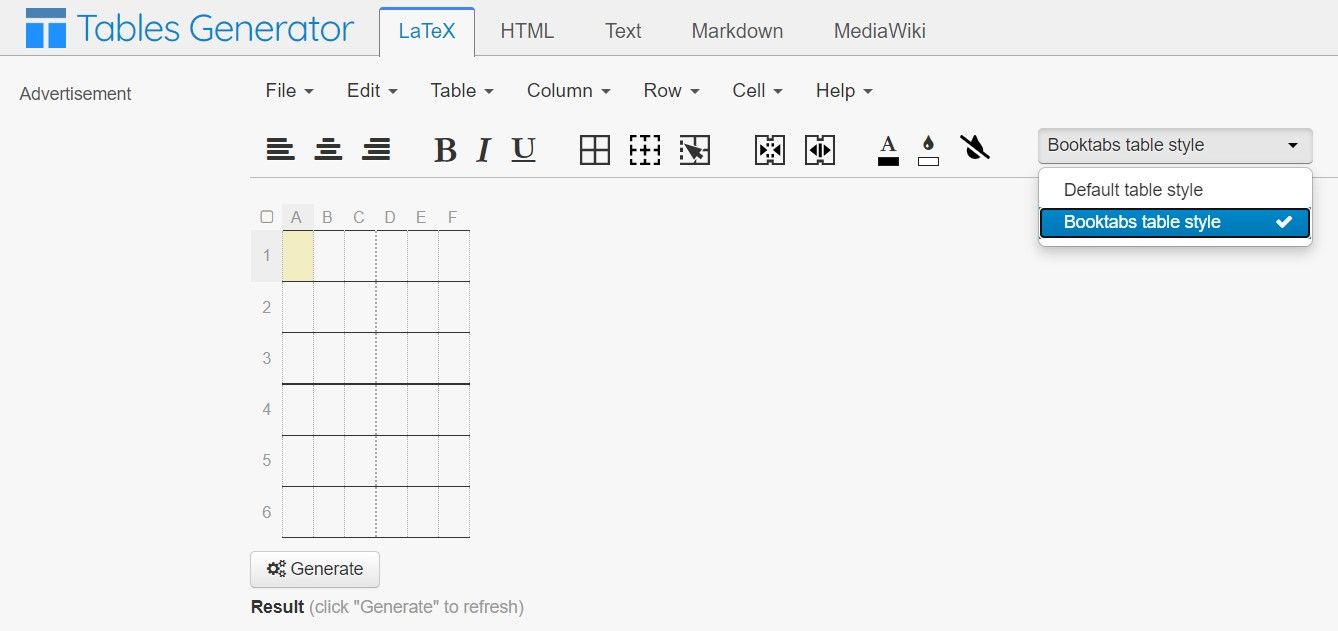
\includegraphics[width=14cm, fbox]{Figures/tablesgenerator.jpg}
\caption{Create a Booktabs style table}
\label{fig:tablegenerator} 
\end{figure}

Use  \texttt{$\backslash$enquote} for double-quotes. \enquote{This is a sample quote.}

Also can try to refer to this image in \autoref{fig:boundingboxexample}. Notice that the \texttt{.eps} and \texttt{.pdf} format vector graphs are favoured, because:

\begin{enumerate}
    \item they can be zoomed-in to check the detail.
    \item text in such formats are search-able.
\end{enumerate}


\begin{figure}[ht]
\centering
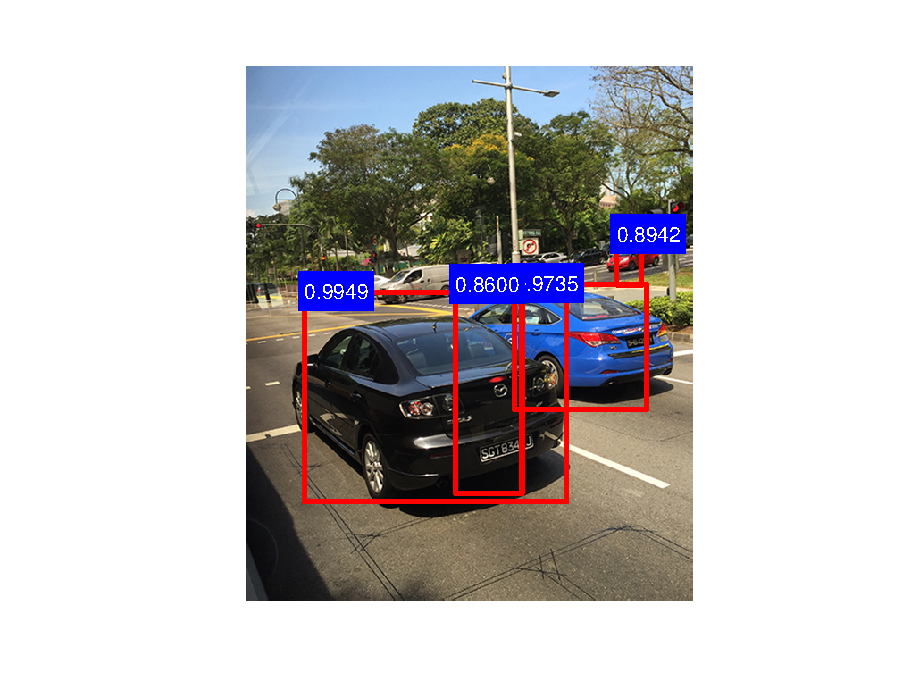
\includegraphics[width=4in, fbox]{Figures/boundingbox.eps}
\caption{Bounding-box example of cars.}
\label{fig:boundingboxexample} 
\end{figure}

Try to insert a math equation as in \autoref{eq:euler}. If you wanna try the in-line mathematical, here is a sample $\alpha = \pi \cdot \frac{1}{\Theta}$.

\begin{equation}
\label{eq:euler}
    e^{ix}= \cos{x} + i \sin{x}
\end{equation}

%Also here is a sample for footnote and hyperlink url\footnote{\url{https://github.com/doem97}}. 

When mention some file formats can use \texttt{music.mp3}, \texttt{latex.pdf}, etc.




\section{Sub-chapter Two}

Contrary to popular belief, Lorem Ipsum is not simply random text. It has roots in a piece of 
\todo{This is a todo note which appears in the margin}
classical Latin literature from 45 BC, making it over 2000 years old. Richard McClintock, a Latin professor at Hampden-Sydney College in Virginia, looked up one of the more obscure Latin words, consectetur, from a Lorem Ipsum passage, and going through the cites of the word in classical literature, discovered the undoubtable source. Lorem Ipsum comes from sections 1.10.32 and 1.10.33 of de Finibus Bonorum et Malorum (The Extremes of Good and Evil) by Cicero, written in 45 BC. This book is a treatise on the theory of ethics, very popular during the Renaissance. The first line of Lorem Ipsum, \enquote{Lorem ipsum dolor sit amet}.., comes from a line in section 1.10.32.

It is a long established fact that a reader will be distracted by the readable content of a page when looking at its layout. The point of using Lorem Ipsum is that it has a more-or-less normal distribution of letters, as opposed to using 'Content here, content here', making it look like readable English. Many desktop publishing packages and web page editors now use Lorem Ipsum as their default model text, and a search for 'lorem ipsum' will uncover many web sites still in their infancy. Various versions have evolved over the years, sometimes by accident, sometimes on purpose (injected humour and the like).

\section{Sub-chapter Three}
\todo[inline]{This todo note appears in line with the text. Todo notes are a great tool to leave comments or notes for self and can then be simply commented out.}
Vivamus eget odio tellus. Nam libero augue, eleifend molestie est eu, tempus vehicula magna. Sed dignissim imperdiet urna, non viverra risus blandit in. In lacinia aliquet leo, ut interdum ipsum ornare sed. Praesent ac fringilla justo. Vivamus pharetra non ipsum eget semper. In hac habitasse platea dictumst. Donec neque lectus, ultricies id massa posuere, sodales interdum ante. Sed et nunc vitae urna ornare porttitor nec vitae urna. Curabitur sit amet luctus urna. Nulla porta malesuada rutrum. Pellentesque vitae velit sed odio tincidunt iaculis. Nulla facilisi.

\newpage

\section{Sub-chapter Four}

To create a bulleted list you need to make use of the ''itemize" environment. A \LaTeX environment is a special section within a page where items as placed. An environment always has a ``\textbackslash{begin}" and a ``\textbackslash{end}". Items you can place in such an environment include:
\begin{itemize}
    \item enumerate -- used to create numbered/letter lists
    \item itemize -- creates a bullet list
    \item figures -- to add images or figures (.eps is the recommended format
    \item tables -- you can create them in tablesgenerator.com then copy the \LaTeX\\code and paste it.
    \item equations -- for those really neat looking mathematical formulae
    \item this list is not exhaustive...
\end{itemize}

\newpage
\section{Sub-chapter Five}
The following are some of the most common commands used during your writing. Some characters are reserved and cannot be directly written as in a normal word processor but need to be ``escaped". Then there are other useful commands such as adding a footnote, inserting a new line (to begin a new paragraph after a blank line, adding labels to items for cross-referencing, etc.

\begin{itemize}
    \item The following are special characters which require a \textbackslash{} before each character so the character is reproduced on the output. The tilde and exponent are even more special. 
    \begin{itemize}
        \item \textbackslash{\#}
        \item \textbackslash{\$}
        \item \textbackslash{\%} -- comment
        \item \textbackslash{\&}
        \item \textbackslash{\_}
        \item \textasciitilde -- type \textbackslash{textasciitilde}
        \item \textasciicircum -- type \textbackslash{textasciicircum}
    \end{itemize}
    \item \textbackslash{textbf} -- bold font
    \item \textbackslash{textit} -- italics
    \item \textbackslash{underline\{words to underline\}}
    \item \textbackslash{emph} -- emphasized text. If used within an italicized text, the output is normal font. If used by itself, text in its argument is italicized.
\end{itemize}
An example highlighting the use of \textbackslash{emph}.
\begin{itemize}
    \item An example of emphasized text with \emph{these words emphasized} within normal font.
    \item \textit{This is an example where \emph{these three words} are emphasized within italicized font}
\end{itemize}

\end{spacing}
%=== END OF CHAPTER ONE ===
\newpage


